\section{Datos y análisis exploratorio}
\label{sec:datos}

\subsection{Corpus e integridad}

El corpus de la competencia contiene 1\,731 tuits etiquetados para
entrenamiento y 1\,154 sin etiquetas de prueba. Cada fila de entrenamiento tiene un
identificador, el texto y tres columnas binarias: HS (discurso de odio), TR
(carácter dirigido) y AG (agresividad). La auditoría de integridad verifica
que no hay valores nulos, que los identificadores son únicos y que se cumple
la regla ontológica de HatEval: en entrenamiento no existe ningún caso con
$TR=1$ y $HS=0$ \cite{basile2019hateval}. Las huellas SHA256 de los tres
archivos oficiales se compararon contra el registro del proyecto antes de
cualquier experimento. El test no se usó para entrenar ni para ajustar el modelo base;
su única función fue generar el envío y alimentar las sondas del leaderboard.

\subsection{Etiquetas, prevalencia y estructura conjunta}

La Tabla~\ref{tab:corpus} resume la distribución. Las tres etiquetas tienen
prevalencias moderadas pero distintas: HS es la más frecuente (43.67\,\%),
AG ocupa una posición intermedia (38.24\,\%) y TR es la minoritaria
(29.98\,\%). La columna TR es, por esa razón, la más frágil: un cambio de una
sola celda pesa más en la métrica que un cambio equivalente en HS. Los
intervalos de Wilson al 95\,\% \cite{wilson1927probable} son estrechos, de
modo que las diferencias de prevalencia no son atribuibles al muestreo.

\begin{table}[t]
\centering
\caption{Distribución de etiquetas y perfiles multietiqueta en entrenamiento
($N=1\,731$). Los intervalos son de Wilson al 95\,\%.}
\label{tab:corpus}
\small
\begin{tabular}{lrrr}
\toprule
Etiqueta / perfil & $n$ & \% & IC95 \\
\midrule
HS & 756 & 43.67 & [41.35, 46.02] \\
TR & 519 & 29.98 & [27.87, 32.18] \\
AG & 662 & 38.24 & [35.98, 40.56] \\
\midrule
000 & 949 & 54.82 & --- \\
001 & 26 & 1.50 & --- \\
100 & 92 & 5.31 & --- \\
101 & 145 & 8.38 & --- \\
110 & 28 & 1.62 & --- \\
111 & 491 & 28.37 & --- \\
\midrule
\multicolumn{4}{l}{\scriptsize * Intervalos de Wilson al 95\,\% para las prevalencias marginales.} \\
\bottomrule
\end{tabular}
\end{table}

Los perfiles multietiqueta muestran una estructura fuertemente condicionada.
Más de la mitad del corpus (949 tuits, 54.82\,\%) es completamente limpio; el
perfil 111 ---las tres etiquetas activas--- concentra 491 casos (28.37\,\%).
No hay ningún caso 010 ni 011: TR solo aparece acompañado de HS. La
agresividad aislada (001) es una rareza: 26 casos, el 1.50\,\%. Esta
observación justifica la regla ascendente $TR=1 \Rightarrow HS=1$ que se aplica
después de la binarización, y descarta la idea de modelar las tres columnas
como si fueran independientes.

La asociación entre etiquetas es alta. El coeficiente $\phi$ vale 0.743
entre HS y TR, 0.831 entre HS y AG y 0.759 entre TR y AG; las tres pruebas
$\chi^2$ rechazan la independencia con $p<10^{-200}$. La estructura es
coherente con la anotación jerárquica de HatEval \cite{basile2019hateval} y con la
literatura sobre clasificación jerárquica \cite{silla2011survey,fortuna2019hierarchically}:
el odio dirigido suele ser también agresivo, y la agresividad sin odio es la
excepción. La Figura~\ref{fig:phi} resume la matriz.

\begin{figure}[t]
\centering
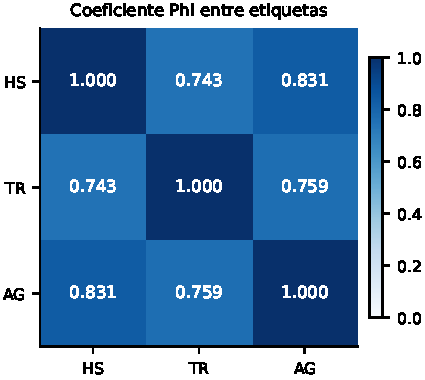
\includegraphics[width=\columnwidth]{fig_phi.pdf}
\caption{Coeficiente $\phi$ entre las tres etiquetas en entrenamiento. Los
valores altos confirman la estructura jerárquica que motiva la regla
$TR=1 \Rightarrow HS=1$.}
\label{fig:phi}
\end{figure}

\subsection{Textometría, ruido y near-duplicados}

Los textos son cortos: la longitud media es de 104.3 caracteres (mediana 91,
máximo 306) y 17.1 palabras (mediana 15). La distribución es asimétrica a la
derecha, con una cola de tuits largos que concentra una parte importante del
error, como se verá en la Sección~\ref{sec:discusion}. El corpus está
normalizado a ASCII: se pierden tildes y eñes, y con ellas parte de la señal
morfológica del español. Esa pérdida es una razón adicional para usar
n-gramas de caracteres, que reconstruyen prefijos, sufijos y variantes
ortográficas sin depender de un diccionario \cite{cavnar1994ngram,mcnamee2004character}.

La búsqueda de near-duplicados sobre la unión de entrenamiento y prueba
(2\,885 textos) encontró cuatro grupos con más de un miembro, un grupo mayor
de seis textos y 17 textos implicados. No es una duplicación masiva, pero
basta para inflar una validación ingenua. Además, se extrajo el pseudo-autor
de cada texto (la primera mención \texttt{@usuario}) y se fusionaron ambos
criterios con una estructura union-find: el entrenamiento queda en 1\,645
grupos, 86 filas menos que la partición por filas. Esa fusión es la unidad de
partición de toda la validación (Sección~\ref{sec:metodologia}). Como control
de fuga por orden, se contrastó la asociación entre el identificador y las
etiquetas: las correlaciones de Spearman fueron $+0.0166$ ($p=0.490$),
$-0.0019$ ($p=0.938$) y $-0.0070$ ($p=0.772$) para HS, TR y AG, y la prueba
$\chi^2$ del identificador agrupado en deciles contra HS dio $\chi^2(9)=12.20$, $p=0.202$. No hay evidencia de que el orden de los identificadores filtre
la etiqueta.

\subsection{Hallazgos que guiaron el modelado}

El análisis exploratorio dejó cinco decisiones estructurales. (i) El
desbalanceo moderado y distinto por etiqueta justifica pesos de clase
balanceados y umbrales desacoplados \cite{japkowicz2002class,lipton2014thresholding}.
(ii) La jerarquía HatEval justifica la regla ascendente. (iii) Los textos
cortos y ruidosos justifican una representación subléxica multiescala.
(iv) Los near-duplicados y los pseudo-autores justifican la validación
agrupada. (v) La ausencia de asociación entre identificador y etiqueta
descarta una fuga por orden. La Figura~\ref{fig:eda} resume los perfiles y
la distribución de longitudes.

\begin{figure*}[t]
\centering
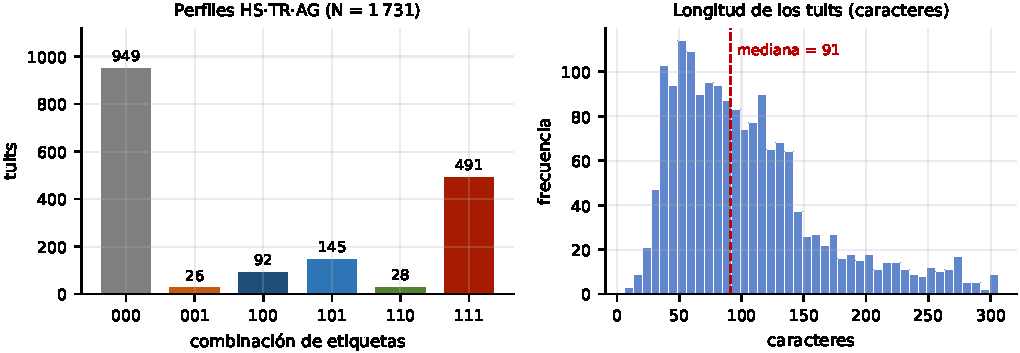
\includegraphics[width=\textwidth]{fig_eda.pdf}
\caption{Análisis exploratorio. Izquierda: perfiles HS$\cdot$TR$\cdot$AG; la
mayoría del corpus es limpio y el perfil 111 es el segundo más frecuente.
Derecha: distribución de longitudes; la mediana es 91 caracteres y la cola
larga concentra los casos más difíciles.}
\label{fig:eda}
\end{figure*}

Una tensión adicional, que no se resuelve con datos, es la definición de TR.
La competencia marca «discurso dirigido contra una persona o grupo»; HatEval
distingue entre objetivo individual y genérico, y exige que el mensaje esté dirigido a uno de ellos
\cite{basile2019hateval}. Varios errores residuales de TR son, en realidad,
desacuerdos de anotación entre esas dos lecturas. Decidimos no modificar las
etiquetas oficiales y modelar la definición de la competencia; la discrepancia
queda documentada como parte del análisis de error.